% 
% Septiembre 2020
% Author: Mathieu Kessler
% Universidad Politécnica de Cartagena
% https://personas.upct.es/perfil/mathieu.kessler
% 
% 
\documentclass[9pt]{beamer}
\definecolor{links}{HTML}{2A1B81}
\hypersetup{colorlinks,linkcolor=,urlcolor=links}
 \usepackage[spanish]{babel}
\usepackage{colortbl}
\usepackage{graphicx}
\usepackage{amsmath,amssymb}
\usepackage{comma}
\usepackage{fancybox,color}
\usepackage[utf8]{inputenc}
\graphicspath{{../figures/}}
\setbeamertemplate{navigation symbols}{}
%\usepackage[colorlinks=true]{hyperref}
\usepackage{xcolor}
\definecolor{mycodecolor}{rgb}{0.65,0.25,0.1}

\usepackage{listings}
\newcommand{\inlinecode}[2][Python]{\lstinline[language=#1, basicstyle=\color{mycodecolor}]{#2}}
\definecolor{mygreen}{rgb}{0,0.6,0}
\definecolor{mygray}{rgb}{0.5,0.5,0.5}
\definecolor{mymauve}{rgb}{0.58,0,0.82}
\lstset{ 
  backgroundcolor=\color{white},   % choose the background color; you must add \usepackage{color} or \usepackage{xcolor}; should come as last argument
  basicstyle=\footnotesize,        % the size of the fonts that are used for the code
  breakatwhitespace=false,         % sets if automatic breaks should only happen at whitespace
  breaklines=true,                 % sets automatic line breaking
  captionpos=b,                    % sets the caption-position to bottom
  commentstyle=\color{mygreen},    % comment style
  deletekeywords={...},            % if you want to delete keywords from the given language
  escapeinside={\%*}{*)},          % if you want to add LaTeX within your code
  extendedchars=true,              % lets you use non-ASCII characters; for 8-bits encodings only, does not work with UTF-8
%  firstnumber=1,                % start line enumeration with line 1000
  %frame=single,	                   % adds a frame around the code
  keepspaces=true,                 % keeps spaces in text, useful for keeping indentation of code (possibly needs columns=flexible)
  keywordstyle=\color{blue},       % keyword style
  language=Python,                 % the language of the code
  morekeywords={*,...},            % if you want to add more keywords to the set
  numbers=left,                    % where to put the line-numbers; possible values are (none, left, right)
  numbersep=5pt,                   % how far the line-numbers are from the code
  numberstyle=\tiny\color{mygray}, % the style that is used for the line-numbers
  rulecolor=\color{black},         % if not set, the frame-color may be changed on line-breaks within not-black text (e.g. comments (green here))
  showspaces=false,                % show spaces everywhere adding particular underscores; it overrides 'showstringspaces'
  showstringspaces=false,          % underline spaces within strings only
  showtabs=false,                  % show tabs within strings adding particular underscores
  stepnumber=2,                    % the step between two line-numbers. If it's 1, each line will be numbered
  stringstyle=\color{mymauve},     % string literal style
  tabsize=2,	                   % sets default tabsize to 2 spaces
  title=\lstname                   % show the filename of files included with \lstinputlisting; also try caption instead of title
}

\usepackage{beamerthemeshadow}
\usepackage{xmpmulti}
\usepackage{mathtools}
\DeclarePairedDelimiter\abs{\lvert}{\rvert}%
\usepackage{tabularx}
\renewcommand\tabularxcolumn[1]{b{#1}}
\newcommand{\field}[1]{\mathbb{#1}}
\newcommand{\E}{\field{E}}
\newcommand{\R}{\field{R}}
\newcommand{\N}{\field{N}}
\newcommand{\Z}{\field{Z}}
\newcommand{\Q}{\field{Q}}
\newcommand{\EE}{\field{E}}
\newcommand{\FF}{\field{F}}
\newcommand{\GG}{\field{G}}
\renewcommand{\L}{\field{L}}
\renewcommand{\P}{\field{P}}
\newcommand{\LL}{{\mathfrak L}}

% define el folder donde del workspace, para cambiar inglés, ids,
% etc..
\newcommand{\workspacefolder}{ids}


\begin{document}
\title{Visual Studio Code: un editor open-source, ligero pero potente}

\author[Mathieu Kessler]{Mathieu Kessler}
\institute[]{Departamento de Matemática Aplicada y Estadística \\ Universidad Politécnica de Cartagena}
\date{\href{https://code.visualstudio.com}{https://code.visualstudio.com}}
\titlegraphic{
\includegraphics[width=3cm]{visual_studio_code_logo}}

\begin{frame}
  \titlepage
\end{frame}

\begin{frame}
  \frametitle{Un editor ligero, rápido y potente}
  \begin{enumerate}
  \item Disponible para  macOS, Linux y Windows
  \item Tiene soporte para cientos de languages de programación
  \item Incluye muchas funcionalides muy útiles como  coloreado de síntaxis,
    balanceado de paréntesis, auto-indentación, selección rectangular,
    capsulas de código.
  \item Permite hacer debugging
  \item Incluye una interfaz para control de versiones (Git)
    
  \item Alto grado de personalización posible, existen muchas extensiones.
  \end{enumerate}
  \pause
  \begin{block}
    
    \begin{center} 
    Se trata de un editor cada vez más popular para Python
    \end{center}
  \end{block}\pause
  \begin{block}{Nota:}
    Visual Studio Code es completamente diferente de  Microsoft Visual
    Studio. No os confundáis!
  \end{block}
\end{frame}
\begin{frame}
  \frametitle{Visual Studio Code está siendo muy popular}
  En la encuesta anual para desarrolladores de  Stack Overflow, hay
  una pregunta sobre editor de texto usado: 
  \begin{center}
    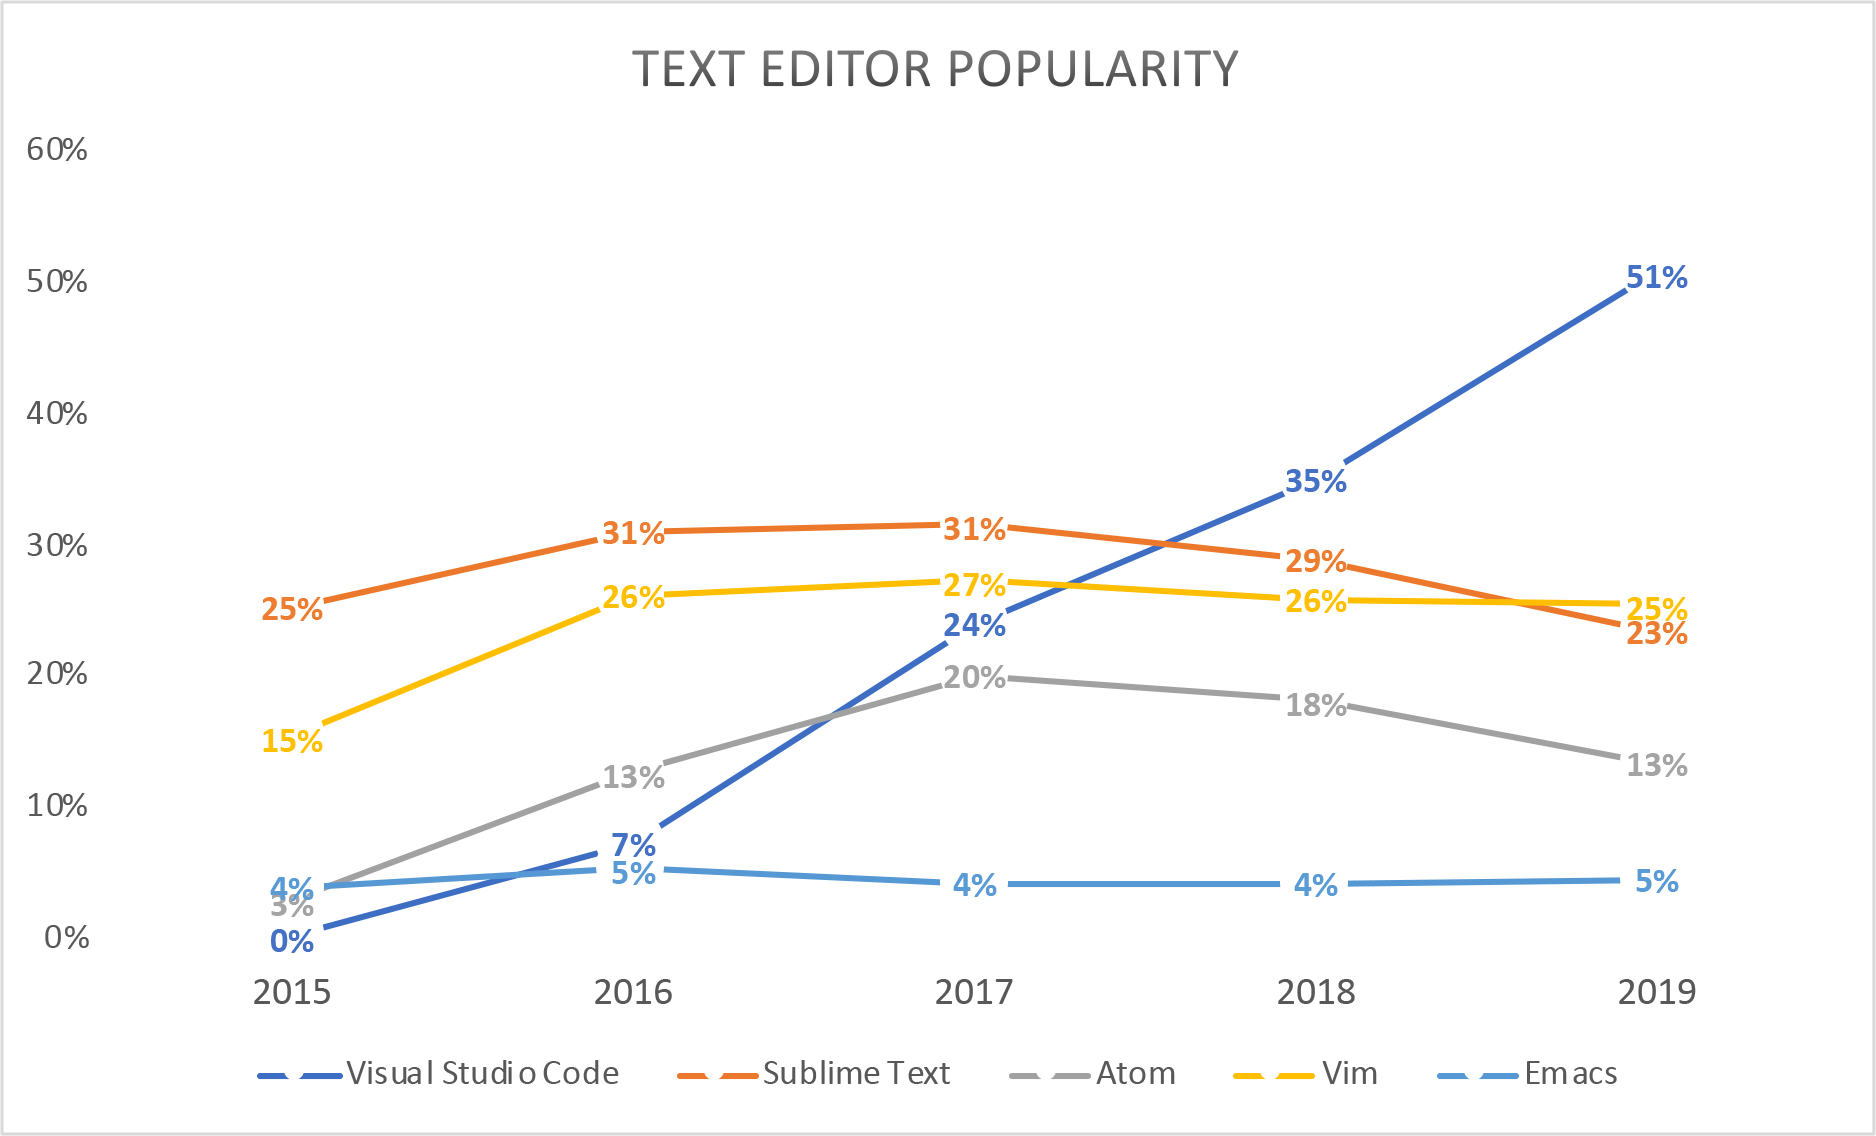
\includegraphics[width=8cm]{2020-09-20-text-editor-popularity}
  \end{center}
  Esta gráfica está extraida del blog post de lectura muy recomendable:
  \textit{The era of Visual Studio Code}, Roben Kleene, 2020-09-21. \href{https://blog.robenkleene.com/2020/09/21/the-era-of-visual-studio-code/}{https://blog.robenkleene.com/2020/09/21/the-era-of-visual-studio-code/}
\end{frame}
\begin{frame}
    \frametitle{Configuración para la asignatura}
          \begin{itemize}
      \item      Descargad y lanzad el ejecutable de instalación de
        \href{https://code.visualstudio.com}{https://code.visualstudio.com}.
    \item Abrid el market place de extensiones a través del icono en
      la barra lateral y buscad la extensión de Python (el autor es el
      propio Microsoft)
                                   \begin{center}
        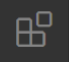
\includegraphics[width=1cm]{extensions_icon.png}\\
        \medskip
        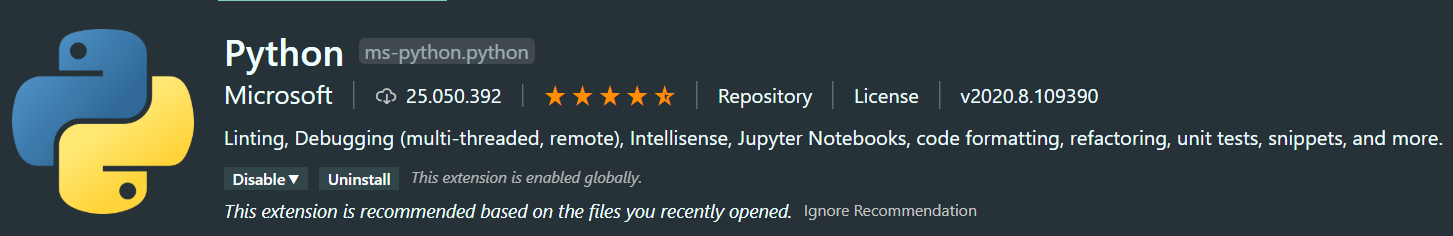
\includegraphics[width=8cm]{python_extension_vscode.png}
                                   \end{center}
                                 \item Cambiaremos el shell por
                                   defecto. Para ello, abrid la paleta
                                   de comandos  (Ctrl - Shift- P),
                                   y teclead  ``Terminal Select
                                   shell''. VS Code lo completará,
                                   escoged la consola estándar.
                                   \begin{center}
                                     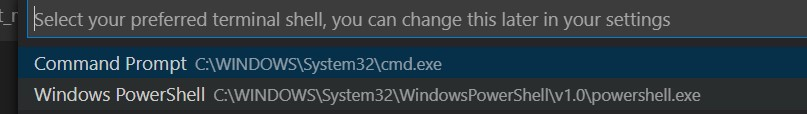
\includegraphics[width=8cm]{select_command_prompt}
                                   \end{center}
                                 \end{itemize}
                               \end{frame}
                               \begin{frame}
        \frametitle{Ahora pasamos a crear un ``workspace''}
        \begin{block}{Workspace en VS Code}
          Un workspace in VS Code es el contenedor para un proyecto,
          incluye todos los ficheros y carpetas relevantes.\\
          Muchas de las opciones de configuración de VS Code se pueden
          establecer a nivel de workspace.          
        \end{block}\medskip
        \pause

        {\huge Pasos:}\medskip
        
        \begin{enumerate}
        \item     En algún lugar en vuestro ordenador, cread la carpeta {\tt
            \workspacefolder}
        \item 
        Desde VS Code, escoged {\tt Add Folder to Workspace}. Esto se
        puede hacer o bien desde el menú  {\tt File} o usando la
        paleta de comandos  (Ctrl - Shift- P) introduciendo ``Add folder''.
      \end{enumerate}
      \pause
      \begin{block}{Nota:}
        Todos los ficheros, programas, datos y figuras asociados a las
        prácticas de esta asignatura se ubicarán en esta carpeta.
        
        \end{block}
        \pause
        Comprobad, usando el icono del explorador
        
\includegraphics[width=.5cm]{explorer_icon.png} en la barra lateral,
        que un workspace sin título se ha creado y que contiene la carpeta {\tt \workspacefolder}.\\
        Podéis guardar el workspace (``Save Workspace as'' en el menú
        File), con el nombre  {\tt \workspacefolder}.
      \end{frame}
    
    \begin{frame}[fragile]
  \frametitle{Creamos nuestro primer proyecto Python}
  Usando el explorador en la barra lateral, hacemos click en la
  carpeta  {\tt \workspacefolder} y creamos una nueva subcarpeta que llamaremos {\tt src}.
  \begin{center}
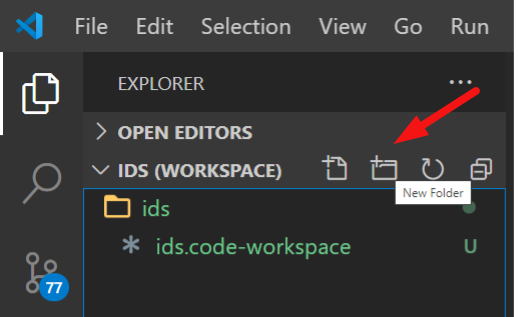
\includegraphics[width=4cm]{vs_code_create_folder}    
  \end{center}
  También creamos una subcarpeta llamada {\tt data} y otra
  llamada {\tt doc}.\\
  La estructura de la carpeta {\tt \workspacefolder} es por lo tanto:
\begin{verbatim}
    ids
        |__ src
        |__ data
        |__ doc
\end{verbatim}
  \begin{block}{Nota}
    \begin{itemize}
    \item     Todos nuestros programas {\tt .py} se ubicarán en la
      carpeta {\tt src} mientras que los blocs de notas estarán en la
      carpeta {\tt doc}.
  \item Todos los ficheros de datos que lleeremos desde Python se
    ubicarán en la carpeta {\tt data}.
    \end{itemize}
    
  \end{block}
\end{frame}
\begin{frame}[fragile]
  \frametitle{Creamos nuestro primer programa Python}
  Usando el Explorador en la barra lateral, haced click en la carpeta
  {\tt src} y cread el fichero {\tt say\_hello.py}.
  \begin{center}
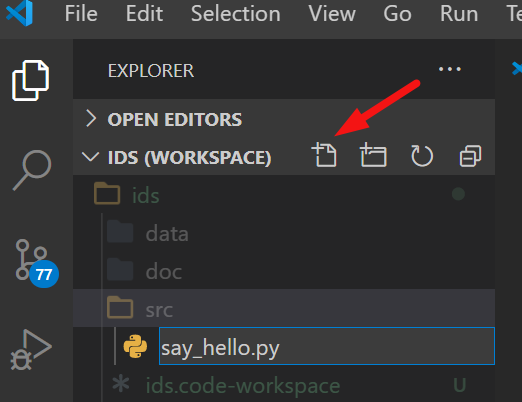
\includegraphics[width=4cm]{vs_code_create_file}    
  \end{center}
  \pause
   La estructura de la carpeta {\tt \workspacefolder} es por lo tanto:
\begin{verbatim}
    ids
        |__ src
        |     |__ say_hello.py
        |
        |__ data
        |__ doc
\end{verbatim}
\end{frame}

\begin{frame}[fragile]
  \frametitle{Creamos nuestro primer program Python}
  En la primer línea de {\tt say\_hello.py}, introducimos
  \begin{lstlisting}
    print('Hello world')
  \end{lstlisting}\vspace{-0.5cm}
  Guardad el fichero. Personalmente tengo la opción de auto-guardado
  activada (Menú File).\\ \smallskip
  \pause
  Para ejecutar el programa, podemos hacer click en el botón de
  ``Play'' en la esquina superior derecha, o desde la paleta de
  comandos, invocar \textit{Python: Run Python file in terminal}.
  \begin{center}
    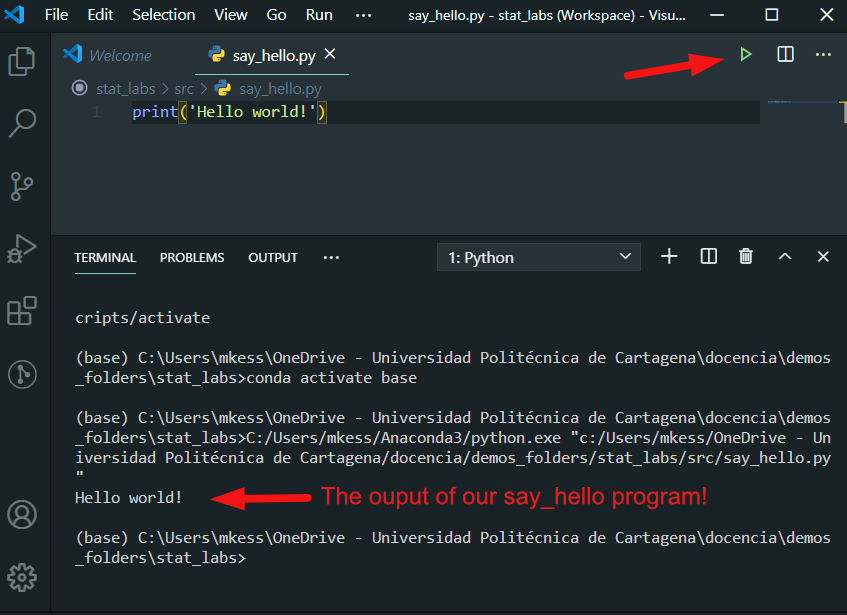
\includegraphics[width=0.7\textwidth]{run_file}
  \end{center}
\end{frame}

\begin{frame}
  \frametitle{Cambiad el entorno virtual}
  \begin{itemize}
  \item   Es una buena práctica trabajar en un entorno virtual. Lo habéis
    tenido que crear ya, siguiendo el documento ``Crear un entorno
    virtual con conda''.
  \item Para cambiarlo para un workspace, podéis
    hacer click en la versión Python de la parte inferior izquierda de
    VS Code o usando la paleta de comandos (Ctrl-Shift-P), introduciendo {\tt Select Interpreter} 
    \begin{center}
      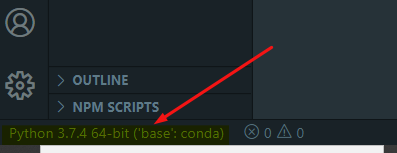
\includegraphics[width=3cm]{change_interpreter_01}
    \end{center}
    Escoged el workspace entero:
    \begin{center}
      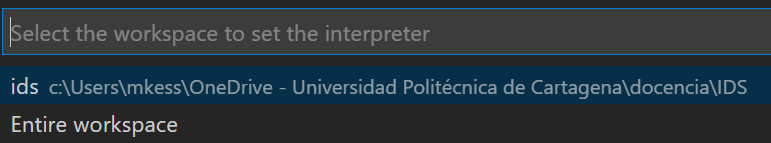
\includegraphics[width=6cm]{change_interpreter_02}
    \end{center}
    y seleccionad el entorno virtual {\tt ids} que habéis creado previamente,    \begin{center}
      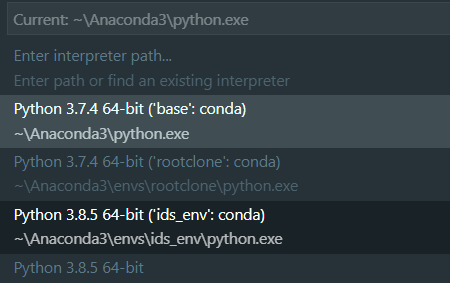
\includegraphics[width=6cm]{change_interpreter_03}
    \end{center}
 
  \end{itemize}
 
\end{frame}

% \begin{frame}
%   \frametitle{Asignar el entorno a nuestro workspace en  Visual Studio Code
%     workspace}
%   \begin{block}{}
%     Ahora que tenemos el Now that our virtual environment {\tt ids} is created, we can
%     assign it to our workspace in Visual Studio Code. 
%   \end{block}
%   To do so, open the course workspace in Visual Studio Code (in previous
%   slides, this workspace was called {\tt stat\_labs}):
%   \begin{itemize}
%   \item In the Command
%     Palette, type ``Select Interpreter''. And choose the entire workspace
%     option
%     \begin{center}
%       \includegraphics[width = 7cm]{select_interpreter_01}
%     \end{center}
%     You can then select the interpreter associated to the {\tt
%       stat\_labs} environment:
%     \begin{center}
%       \includegraphics[height = 2cm]{select_interpreter_02}
%     \end{center}
%   \end{itemize}
% \end{frame}
\begin{frame}
  \frametitle{Para comprobar que se ha seleccionado correctamente el entorno}
  Podéis comprobar que el entorno {\tt ids} está activado en la parte
  izquierda de la barra inferior:
  \begin{center}
      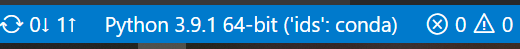
\includegraphics[width=4cm]{check_interpreter_01}
  \end{center}\pause
  O podéis abrir un nuevo  terminal  (Terminal menu $\leftarrow$ New
  Terminal), y podéis comprobar que conda activa el entorno {\tt ids } :
  \begin{center}
      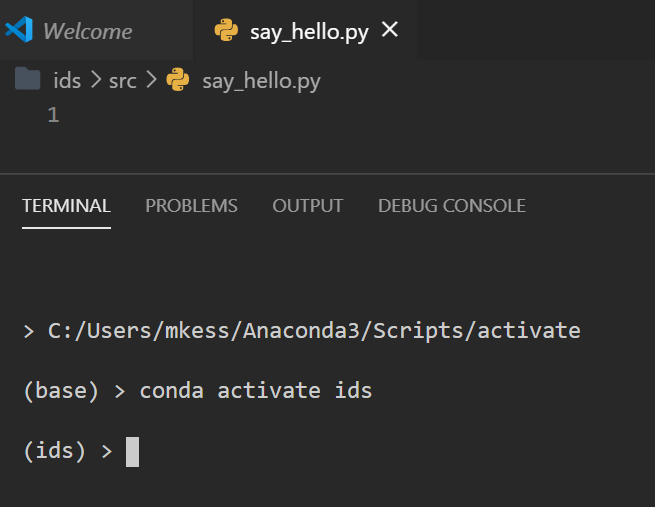
\includegraphics[height=5cm]{check_interpreter_02}
  \end{center}	
\end{frame}
\end{document}


\begin{frame}
  \frametitle{Par ejecutar una sesión interactiva de Python}
  Tenemos dos opciones:
  \begin{enumerate}
  \item Desde el menú ``Terminal'', escoged  ``New Terminal''. Una
    consola se abre. Podéis entonces teclear
    \inlinecode[bash]{python} para lanzar una sesión interactiva de
    Python.
    
  \item Creando una ventana interactiva desde la paleta de comandos: :
    \textit{Python: Create Python Interactive Window}
    \begin{center}
      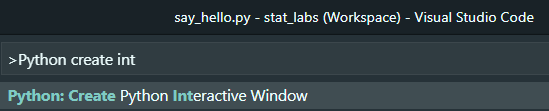
\includegraphics[width=5cm]{create_interactive_windows_01}
    \end{center}
    Podéis introducir y ejecutar código en las celdas
    \begin{center}
      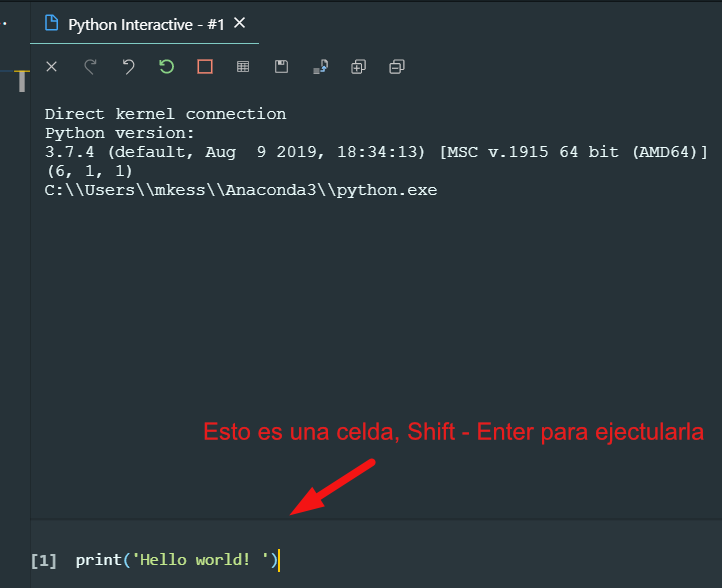
\includegraphics[width=5.5cm]{create_interactive_windows_02-es}
    \end{center}
  \end{enumerate}
\end{frame}
\end{document}

